%plurals_event
%PRECOMPILE COMMAND pdftex -ini -jobname="plurals_event_chap_34" "&pdflatex" mylatexformat.ltx plurals_event_chap_34.tex
\documentclass[english]{article}
\usepackage[T1]{fontenc}
\usepackage[latin1]{inputenc}
\usepackage[sort]{natbib}
\usepackage{stdprmbl}

\usepackage{parskip}

\lingset{interpartskip = -5pt}
\lingset{aboveexskip = 3pt,belowexskip = 3pt, belowpreambleskip = -3pt}

\definecolor{darkred}{rgb}{0.7,0,0}
\definecolor{blueish}{rgb}{0,0,0.7}
\newcommand{\ag}{\textsc{Agent}\xspace}
\newcommand{\thm}{\textsc{Theme}\xspace}
\newcommand{\goal}{\textsc{Goal}\xspace}

\newcommand{\fg}{\color{darkred}}
\newcommand{\bg}{\color{blueish}}


% \endofdump

\newcommand{\scale}{1}

\title{Plurals and events (chap. 9) : Cumulative quantification}
\author{Keny Chatain}

\begin{document}
\maketitle

This chapter is the grand finale I've eagerly been waiting for.

\section{Introduction}

\paragraph{The problem in a nutshell.}

In this section, Schein starts by outlining the problem of cumulative readings with modified numerals.

\pex
\a
Two detectives solved three crimes.
\a 
Less than two detectives solved less than 3 crimes. \label{detectives}
\xe
%
Schein notes that both sentences give rise to scopeless truth-conditions ; it isn't clear that either quantifier can be said to scope above the other. Despite this intuition, \clastxa can be given a logical representation in which one quantifier scopes above the other \cnextxa ; this is completely equivalent to a symmetrical logical representation where the opposite scope relation holds \cnextxb

\pex
\a 
$\exists X\in \textsf{2-detectives}, \exists Y\in \textsf{3-detectives},$ $X$ solved $Y$
\a
$\exists Y\in \textsf{3-detectives}, \exists X\in \textsf{2-detectives},$ $X$ solved $Y$
\xe
%
This fortunate scopelessness of the representation unfortunately does not hold for \cref{detectives}. Each gives rise to its own \emph{pseudo-cumulative} reading and neither reading are attested. We need a non-accidental way to generate scopelessness.

\pex
\a 
$<2\ X \in\textsf{detectives}, <3\ Y \in\textsf{crimes},$ $X$ solved $Y$\\
$\leftrightsquigarrow$\emph{the groups of detectives whose total crime score is less than 3 have less than 2 members}
\a 
$<3\ Y \in\textsf{crimes}, <2\ X \in\textsf{detectives}, $ $X$ solved $Y$
\xe
%
 Schein notes that this problem is not tied to assuming plural objects since his essentially equivalent LFs will also generate pseudo-cumulative reading.

\paragraph{The solution in a nutshell.} Schein proposes that at LF, the two quantifiers merge to form a binary object. The intended translation of these exotic LFs into logical formulas is in terms of an anaphoric dependency with two conjuncts

\pex
\a 
Less than two detectives reported less than 3 crimes to less than 2 agencies. 
\a 
\textbf{LF:}\\
%!TEX root = ../plurals_event_chap_9.tex
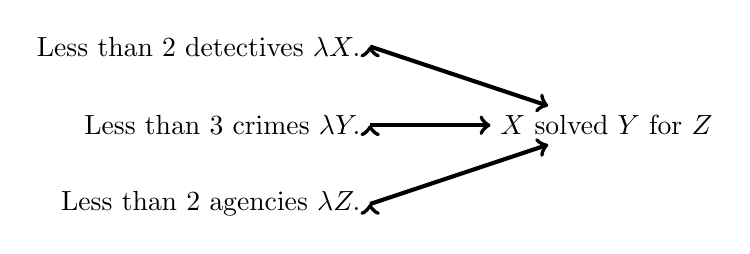
\begin{tikzpicture}[scale = \scale, baseline = {([yshift={-\ht\strutbox}]current bounding box.north)}]
\node[anchor = east] (v1) at (-3,1.5) {Less than 2 detectives $\lambda X.$};
\node[anchor = east] (v3) at (-3,0.5) {Less than 3 crimes $\lambda Y.$};
\node[anchor = east] (v4) at (-3,-0.5) {Less than 2 agencies $\lambda Z.$};
\node (v2) at (0,0.5) {$X$ solved $Y$ for $Z$};
\draw [->,line width = 1.5pt] (v1.east) edge (v2);
\draw [->, line width = 1.5pt] (v3.east) edge (v2);
\draw [->, line width = 1.5pt] (v4.east) edge (v2);
\end{tikzpicture}
\a \textbf{Logical formula:}\\
{\bg $[<2\ X \in\textsf{detectives}, \exists Y\in\textsf{crimes}, \exists Z\in\textsf{agencies},$\\
$\ag(E) = X \wedge \thm(E) = Y \wedge \goal(E) = Z \wedge \textsf{solved}(E)]^{73}$}\\[1ex]
{\fg $\wedge [\iota E: E = \text{pro}_{73},  <3\ Y\in\textsf{crimes}, \thm(E) = Y \wedge \textsf{solved}(E)]$\\
$\wedge [\iota E: E = \text{pro}_{73},  <3\ Z\in\textsf{agencies}, \goal(E) = Z \wedge \textsf{solved}(E)]$
}
\a \textbf{Schein's paraphrase:}\\
\emph{
Less than two detectives reported crimes to agencies\\
and there, less than 3 crimes were reported\\
and there, to less than 2 agencies were crimes reported
}
\xe
%
The logical formula has two parts: a {\bg conjunct} that introduces an antecedent ensemble event  which the subsequent {\fg conjuncts} further describe. In the subsequent section, Schein sets out to justify the exact shape of the logical formula he assumes:

\begin{itemize}
	\item \emph{Anaphora:} conjuncts related by anaphoric dependencies
	\item \emph{Cumulative asymmetry:} one quantifier is selected to belong to the clause that introduces the event referent
\end{itemize}
%
The event DR introduction is observed to follow the general rules of DR introduction ; it always introduce a maximal referent:


\section{Why cumulativity must be asymmetric}

This first section is devoted to justify the \emph{cumulative asymmetry}. This is a surprising feature of the analysis as the paraphrase of the truth conditions seem completely symmetric in the quantifiers that enter the relations:

\pex
\a 
Less than 3 detectives solved less than 5 crimes
\a \textbf{TCs:}\\
\emph{less than 3 detectives solved crimes}\\
\emph{less than 5 crimes were solved}
\xe
%
However, Schein wishes to suggest that the symmetric truth-conditions is inadequate for the more complex case in \cnextx:

\pex
\a 
Exactly two detectives each solved exactly two crimes for exactly 3 agencies
\a 
Exactly two detectives each solved exactly two crimes for exactly 1 agencies
\xe
%
The intended reading is one where:

\begin{itemize}
 	\item \emph{the crimes} is interpreted distributively relative to \emph{the detectives}
 	\item \emph{the detectives} and \emph{the agencies} enter a cumulative relation
 \end{itemize} 
%
For instance, we can note that \clastxa will be true and \clastxb will be false in the scenario below:

\ex
%!TEX root = ../plurals_event_chap_9.tex
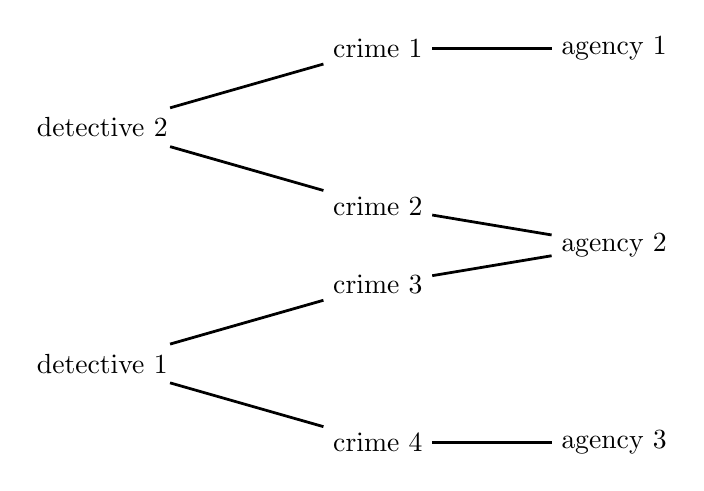
\begin{tikzpicture}[scale = \scale, baseline = {([yshift={-\ht\strutbox}]current bounding box.north)}]
\node (v1) at (2.5,2.5) {agency 1};
\node (v2) at (-0.5,2.5) {crime 1};
\node (v4) at (-0.5,0.5) {crime 2};

\node (v5) at (2.5,0) {agency 2};
\node (v6) at (-0.5,-0.5) {crime 3};
\node (v7) at (2.5,-2.5) {agency 3};
\node (v8) at (-0.5,-2.5) {crime 4};
\node (v3) at (-4,1.5) {detective 2};
\node (v9) at (-4,-1.5) {detective 1};
\draw [line width  = 1pt] (v2) edge (v1);
\draw [line width  = 1pt] (v4) edge (v5);
\draw [line width  = 1pt] (v6) edge (v5);
\draw [line width  = 1pt] (v8) edge (v7);
\draw [line width  = 1pt] (v9) edge (v6);
\draw [line width  = 1pt] (v9) edge (v8);
\draw [line width  = 1pt] (v4) edge (v3);
\draw [line width  = 1pt] (v3) edge (v2);
\end{tikzpicture}
\xe
%
Symmetric paraphrases:

\pex
\a 
Exactly two detectives each reported exactly two crimes to agencies\\
To exactly three agencies did detectives report exactly two crimes\\
\a 
Exactly two detectives each reported exactly two crimes to agencies\\
To exactly three agencies did detectives report exactly two crimes\\
\xe
%
\begin{squ}
The sentence is true because there is exactly one agency that detectives reported exactly two crimes for.
\end{squ}
%
However, it seems that this symmetric paraphrase is missing the \emph{each} operator that yields the correct reading. Not sure that Schein's argument goes through once we reestablish that:

\pex
\a 
Exactly two detectives each reported exactly two crimes to agencies\\
To exactly three agencies did detectives \textbf{each} report exactly two crimes\\
\a 
Exactly two detectives each reported exactly two crimes to agencies\\
To exactly three agencies did detectives \textbf{each} report exactly two crimes\\
\xe
%

\section{What is the reference of the event anaphor}

\paragraph{Analogy with anaphors}
Schein's paraphrase of cumulative sentences involves an event anaphor, depicted as \emph{there}. 

\pex
\a 
Less than two detectives reported less than 3 crimes. 
\a \textbf{Schein's paraphrase:}\\
\emph{
Less than two detectives reported crimes\\
and there, less than 3 crimes were reported
}
\xe
%
For this paraphrase to go through, it would seem that \emph{there} should refer to all the events of reporting crimes to agencies by detectives. How does \emph{there} get to refer to this particular sets of events?

Schein's interesting observation is that there is no difference between event anaphors and anaphors to individuals, so whatever we need to say about the former is whatever we need to say about the latter. In particular, the following parallel is telling:

\definecolor{darkorange}{HTML}{efc67c}
\definecolor{bluegray}{HTML}{b1d1ed}
\definecolor{purple}{HTML}{ba83c4}
\pex
\a 
{\color{darkorange!84!black} Less than 3 farmers} bought {\fg a donkey}.\\
{\color{purple!93!black} They} carried {\color{bluegray!93!black} less than 4 bags of oats}.
\a 
{\color{darkorange!84!black} Less than 3 farmers} {\fg $\exists e$} bought donkeys.\\
{\color{purple!93!black} There,} {\color{bluegray!93!black} less than four donkeys} were bought.
\xe
%
In particular, he notes that in cross-clausal subordination contexts, there seems to be a difference in the reading of the anaphor depending on the nature of the subordinator\footnote{This data point, if genuine, is an added dimension to the problem of weak/strong reading in anaphors. In particular, it shows a weak/strong ambiguity look-alike that is not dependent on the monotonicity of the \emph{anaphor}'s environment (contra Kanazawa).}.

\pex
\a 
Few farmers bought a donkey\ldots\\
\ldots they hitched them together to a mule train.\\
\emph{they refers to all the bought donkeys}
\a 
Every farmer bought a donkey\ldots\\
\ldots they hitched them together to a mule train.\\
\emph{they refers to a plurality of one bought donkey per farmer}
\xe
%
So quantifiers like \emph{few} seem to impose maximal readings of the anaphors and while \emph{every} delivers non-maximal readings. This difference is claimed to be observable in event anaphor cross-reference as well:

\pex
\a 
In ten minutes, every farmer fed a donkey.
\a 
Every farmer $\exists e$ fed a donkey.\\
There, farmers fed donkeys in ten minutes\\
\emph{there refers to an event plurality containing one event per farmer}
\xe
%
A minimal pair with \emph{few} is lacking in the book. If we construct it, I am not certain that the reading we get is teh exact counterpart of \clastx 
\ex
In ten minutes, few farmers fed a donkey.
\xe
%
Not looking for a minimal pair, we already know that for cumulative sentences, \emph{there} must refer to all the buying events by a farmer, confirming the maximality already observed:

\ex
{\color{darkorange!84!black} Less than 3 farmers} bought {\fg a donkey}.\\
{\color{purple!93!black} They} carried {\color{bluegray!93!black} less than 4 bags of oats}.
\xe

\paragraph{Meandering aimlessly.} Schein get a bit stuck in his paraphrases because he is regrettably married to the idea that anaphors must be resolved as definite descriptions. 

\pex
{\bg Exactly two farmers}\textsubscript{56} each fed {\fg two donkeys}\textsubscript{89} {\color{purple} one bag of oats}\textsubscript{32}.\\
\a 
they\textsubscript{89} $\neq$ \emph{the donkeys that farmers fed bags of oats to}\\
they\textsubscript{89} $\neq$ \emph{the donkeys that the farmers fed one bag of oats to}
\a 
%!TEX root = ../plurals_event_chap_9.tex
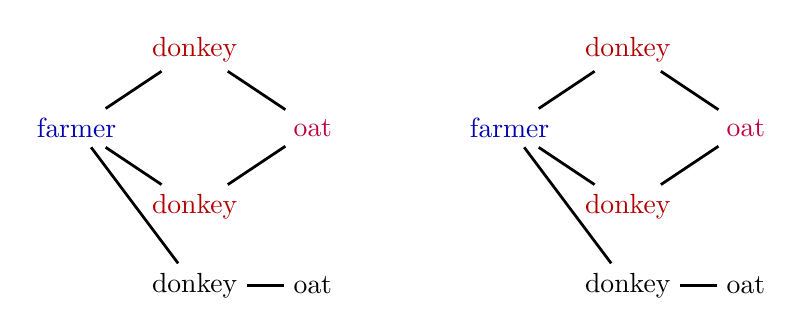
\begin{tikzpicture}[scale = \scale, baseline = {([yshift={-\ht\strutbox}]current bounding box.north)}]
\node (v2) at (-3,1.5) {\fg donkey};
\node (v3) at (-3,-0.5) {\fg donkey};
\node (v5) at (-1.5,0.5) {\color{purple} oat};
\node (v7) at (1,0.5) {\bg farmer};
\node (v8) at (2.5,1.5) {\fg donkey};
\node (v9) at (2.5,-0.5) {\fg donkey};
\node (v10) at (4,0.5) {\color{purple} oat};
\node (v1) at (-4.5,0.5) {\bg farmer};

\node (v4) at (-3,-1.5) {donkey};
\node (v6) at (-1.5,-1.5) {oat};
\node (v11) at (2.5,-1.5) {donkey};
\node (v12) at (4,-1.5) {oat};

\draw [line width = 1pt] (v1) edge (v2);
\draw [line width = 1pt] (v1) edge (v3);
\draw [line width = 1pt] (v1) edge (v4);
\draw [line width = 1pt] (v3) edge (v5);
\draw [line width = 1pt] (v2) edge (v5);
\draw [line width = 1pt] (v4) edge (v6);
\draw [line width = 1pt] (v7) edge (v8);
\draw [line width = 1pt] (v7) edge (v9);
\draw [line width = 1pt] (v8) edge (v10);
\draw [line width = 1pt] (v9) edge (v10);
\draw [line width = 1pt] (v7) edge (v11);
\draw [line width = 1pt] (v12) edge (v11);
\end{tikzpicture}
\xe
%
The correct definite descriptions are undesirable for Schein:

\begin{squ}
There ought to be more to the explanation of cumulative reference than an algorithm that introduces indefinite descriptions ad hoc into an already elaborate notion of descriptive content.
\end{squ}

\section{Rendering}

The solution is to adapt some vehicle for discourse referents, some entity which can hold all the entities that need to be transmitted to the next clause. Schein could have chosen assignments as in DS, or situations as in Heim/Elbourne E-type  theories. He chooses naturally to make events his DR vehicle\footnote{He calls his vehicle \emph{states of affair}, borrowing from Barry Taylor.} This is called \emph{rendering}: $E$ render a sentence $S$ if $E$ is the DR vehicle made available by $S$

Just as DS defines CCPs in a lexicalized manner, Schein defines for each operator in his logical formulas, the DR event that it introduces (i.e. the event that it renders). Here are some definitions:

\ex
\begin{tabular}[t]{ll}
  E renders $\Theta (X, E')$
  \\
  \emph{iff}
  \\
  $E$ is the set of events whose $\Theta$ is X\footnotemark
\end{tabular} 
\footnotetext{
I'm suppressing reference to complete overlap for simplicity (cf chap 4).
}
\xe
%
\ex~
\begin{tabular}[t]{ll}
E renders $Q x: \Phi(x), \Psi(x)$
\\
\emph{iff}
\\
$E= \left\lbrace e\text{ renders }\Psi(x)\ \middle|\ x\in\Phi\right\rbrace$
\end{tabular} 
\xe
%
\ex~ \label{exist}
\begin{tabular}[t]{ll}
E renders $\exists E: \Phi(E), \Psi(E)$
\\
\emph{iff}
\\
$E\in \Phi\cap\Psi$
\end{tabular} 
\xe
%
The latter two denotations are close relatives with the corresponding DS denotation. For quantifiers, the DRs introduced in each true quantificational case are gathered together in one big DR ; for existentials, any witness would do. With this, we are ready to confront the donkey problem seen earlier:

\pex
{\bg Exactly two farmers}\textsubscript{56} each fed {\fg two donkeys}\textsubscript{89} {\color{purple} one bag of oats}\textsubscript{32}.
\a 
\begin{tabular}[t]{ll}
they\textsubscript{89} & $\neq$ \emph{the donkeys that the farmers fed one bag of oats to}\\
 & $=$ \emph{the theme donkeys in the events that render \cnextxa}
\end{tabular}
\a 
%!TEX root = ../plurals_event_chap_9.tex
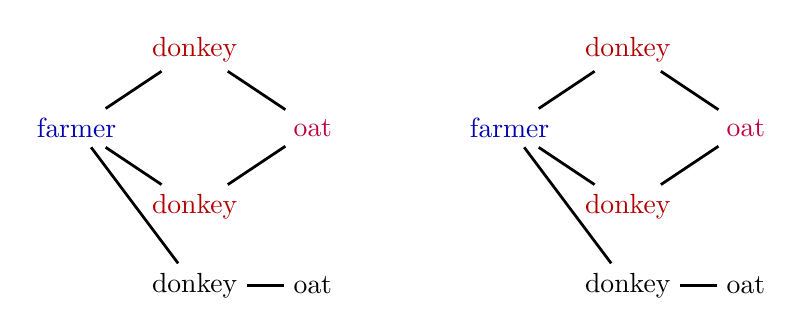
\begin{tikzpicture}[scale = \scale, baseline = {([yshift={-\ht\strutbox}]current bounding box.north)}]
\node (v2) at (-3,1.5) {\fg donkey};
\node (v3) at (-3,-0.5) {\fg donkey};
\node (v5) at (-1.5,0.5) {\color{purple} oat};
\node (v7) at (1,0.5) {\bg farmer};
\node (v8) at (2.5,1.5) {\fg donkey};
\node (v9) at (2.5,-0.5) {\fg donkey};
\node (v10) at (4,0.5) {\color{purple} oat};
\node (v1) at (-4.5,0.5) {\bg farmer};

\node (v4) at (-3,-1.5) {donkey};
\node (v6) at (-1.5,-1.5) {oat};
\node (v11) at (2.5,-1.5) {donkey};
\node (v12) at (4,-1.5) {oat};

\draw [line width = 1pt] (v1) edge (v2);
\draw [line width = 1pt] (v1) edge (v3);
\draw [line width = 1pt] (v1) edge (v4);
\draw [line width = 1pt] (v3) edge (v5);
\draw [line width = 1pt] (v2) edge (v5);
\draw [line width = 1pt] (v4) edge (v6);
\draw [line width = 1pt] (v7) edge (v8);
\draw [line width = 1pt] (v7) edge (v9);
\draw [line width = 1pt] (v8) edge (v10);
\draw [line width = 1pt] (v9) edge (v10);
\draw [line width = 1pt] (v7) edge (v11);
\draw [line width = 1pt] (v12) edge (v11);
\end{tikzpicture}
\xe
%
Note that Schein is still married to E-type descriptions. He gives one reason why: definite descriptions introduce maximality, which Evans argues is desirable for definite descriptions.

\pex
\a John owns some sheep\textsubscript{63}.
\a Harry vaccinated them\textsubscript{63}.
\xe
%
By the denotation in \cref{exist}, the events that render \clastxa true are any events of John owning sheep.  The definite description in \clastxb will only pick out the maximal event that renders \clastxa true. This way, we ensure that all the sheep owned by John were vaccinated. This is a different division of labor than is usually found in DS. In DS, maximality is introduced at the level of the pronoun rather than its antecedent\footnote{Difficult to know whether this is preferable to the DS way of doing things. If we adopt a Heim (1982, chap 1) way of doing donkey sentences, then the sentence in \cnextxa may be predicted to have the reading in \cnextxb if maximality is only introduced at the level of the pronoun.

\pex
\a 
Every farmer who owns donkeys drew a circle around them\\
\a 
Drew a circle around each subgroup of donkeys.
\xe
%
But there may be other ways of doing donkeys with Schein's tools.
}.

\paragraph{DE quantifiers.} Downward entailing quantifiers are compatible with a situation with no witness, hence no rendering event. Yet, that does not result in problematic truth-conditions.

\pex
\a 
Less than 3 detectives each solved exactly two crimes for less than three agencies.
\a 
\textbf{Schein's paraphrases:}\\
\emph{[less than 3 detectives solved crimes for agencies]\textsubscript{78}}\\
\emph{there\textsubscript{78}, detectives solved crimes for less than three agencies}
\xe
%
%!TEX root = ../plurals_event_chap_9.tex
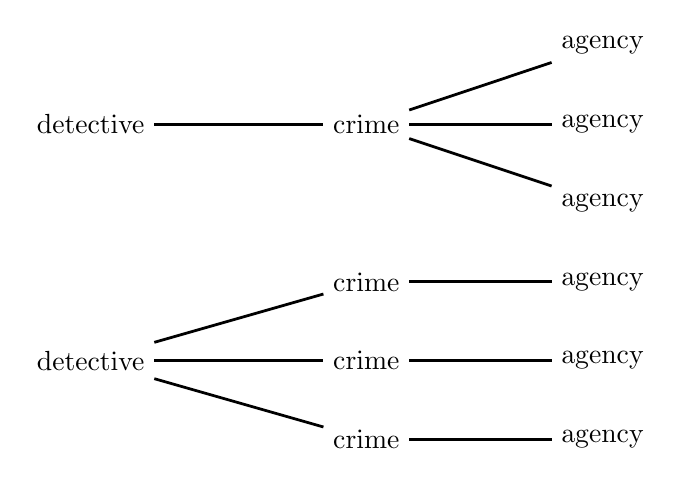
\begin{tikzpicture}[scale = \scale, baseline = {([yshift={-\ht\strutbox}]current bounding box.north)}]

\node (v3) at (2.5,2.5) {agency};
\node (v12) at (2.5,0.5) {agency};
\node (v6) at (2.5,-0.5) {agency};
\node (v8) at (2.5,-1.5) {agency};
\node (v10) at (2.5,-2.5) {agency};
\node (v4) at (2.5,1.5) {agency};

\node (v2) at (-0.5,1.5) {crime};
\node (v5) at (-0.5,-0.5) {crime};
\node (v7) at (-0.5,-1.5) {crime};
\node (v9) at (-0.5,-2.5) {crime};

\node (v1) at (-4,1.5) {detective};
\node (v11) at (-4,-1.5) {detective};



\draw [line width = 1pt] (v2) edge (v3);
\draw [line width = 1pt] (v2) edge (v4);
\draw [line width = 1pt] (v5) edge (v6);
\draw [line width = 1pt] (v7) edge (v8);
\draw [line width = 1pt] (v9) edge (v10);
\draw [line width = 1pt] (v11) edge (v5);
\draw [line width = 1pt] (v11) edge (v7);
\draw [line width = 1pt] (v11) edge (v9);
\draw [line width = 1pt] (v1) edge (v2);
\draw [line width = 1pt] (v2) edge (v12);

\end{tikzpicture}


\end{document}
